%!TEX root = ../master.tex

\section{External powers attacking the consumer}
In \cref{applianceCompanyTree} some more distant powers were mentioned - countries, terrorist organisations, environmental activists and blackmailers.
Common for these is that they are very distant to the consumer and they do not need to know much about the consumer as an individual.
Abusing the smart meter of the consumer is a means to an end in a much bigger perspective.

They all want to shut down the power of the consumer in order to achieve a bigger objective, power, political influence or money.
The posibilities enabled by an offswitch were discussed in \cref{off_switch}.
The attack tree depicting this simple attack can be seen on \cref{fig:attack_trees:external}.

\begin{figure}[h]
  \centering
	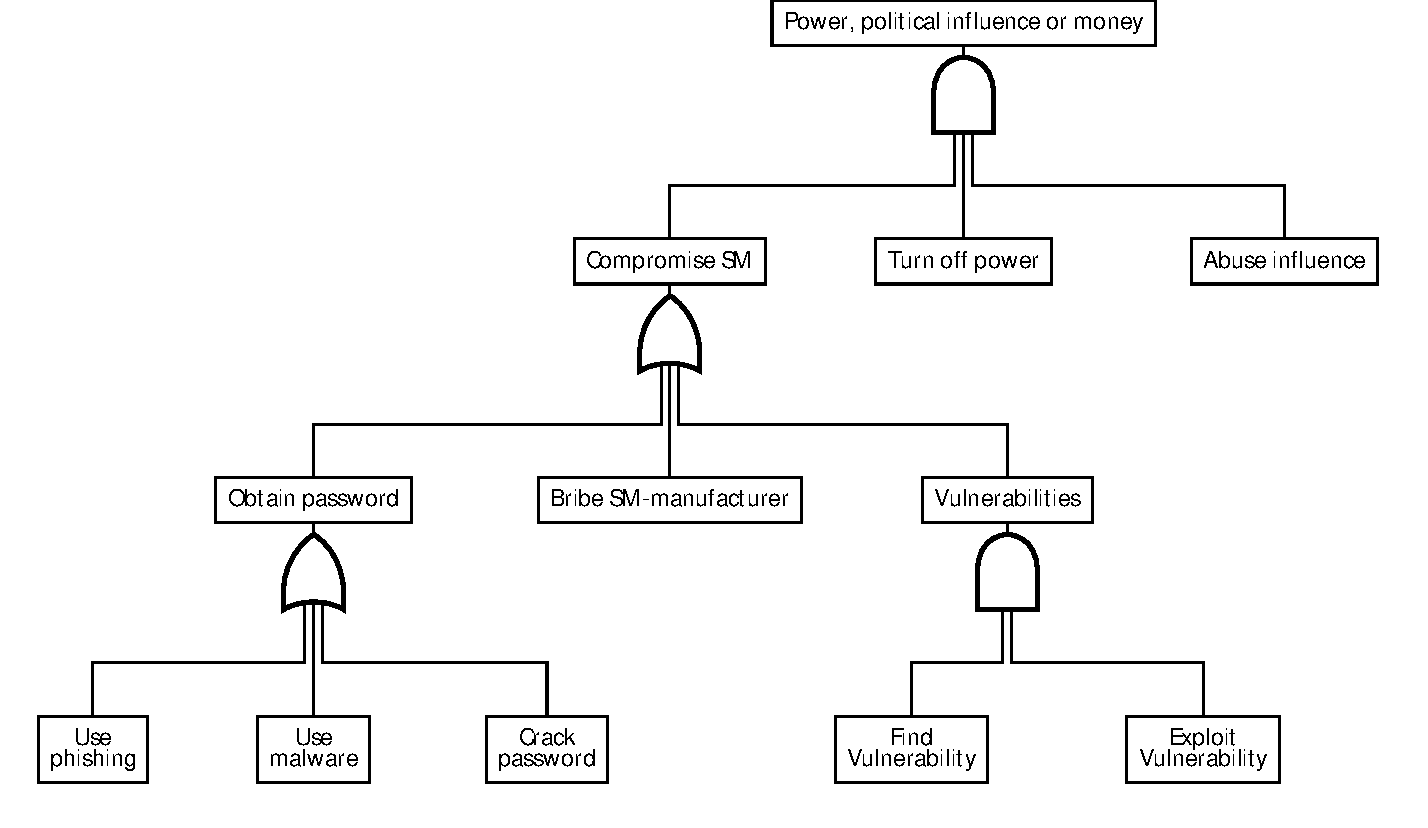
\includegraphics[width=.75\textwidth]{figures/graphviz/offswitch.pdf}
	\caption{External powers attacking the consumer.}
	\label{fig:attack_trees:external}
\end{figure}